\chapter{การติดตั้งเครื่องมือที่ใช้พัฒนาโปรแกรม}
การติดตั้งเครื่องมือที่ใช้ในการพัฒนาแอปพลิเคชันระบบกองทุนเงินให้กู้ยืมเพื่อการศึกษา คณะวิทยาศาสตร์ มหาวิทยาลัยอุบลราชธานี มีโปรแกรมที่จำเป็นในการพัฒนาระบบดังต่อไปนี้
\begin{itemize}
	\item การติดตั้ง Android Studio
	\item การติดตั้ง Node.js
	\item การติดตั้ง Vue.js Fronted Framwork
\end{itemize}

\section{การติดตั้ง Android Studio}
\begin{enumerate}
	\item สามารถดาวน์โหลด Android Studio installer package ได้ที่ https://developer.android.com/studio/ ดังแสดงในรูปที่ \ref{Fig:android1}
	\begin{figure}[H]
		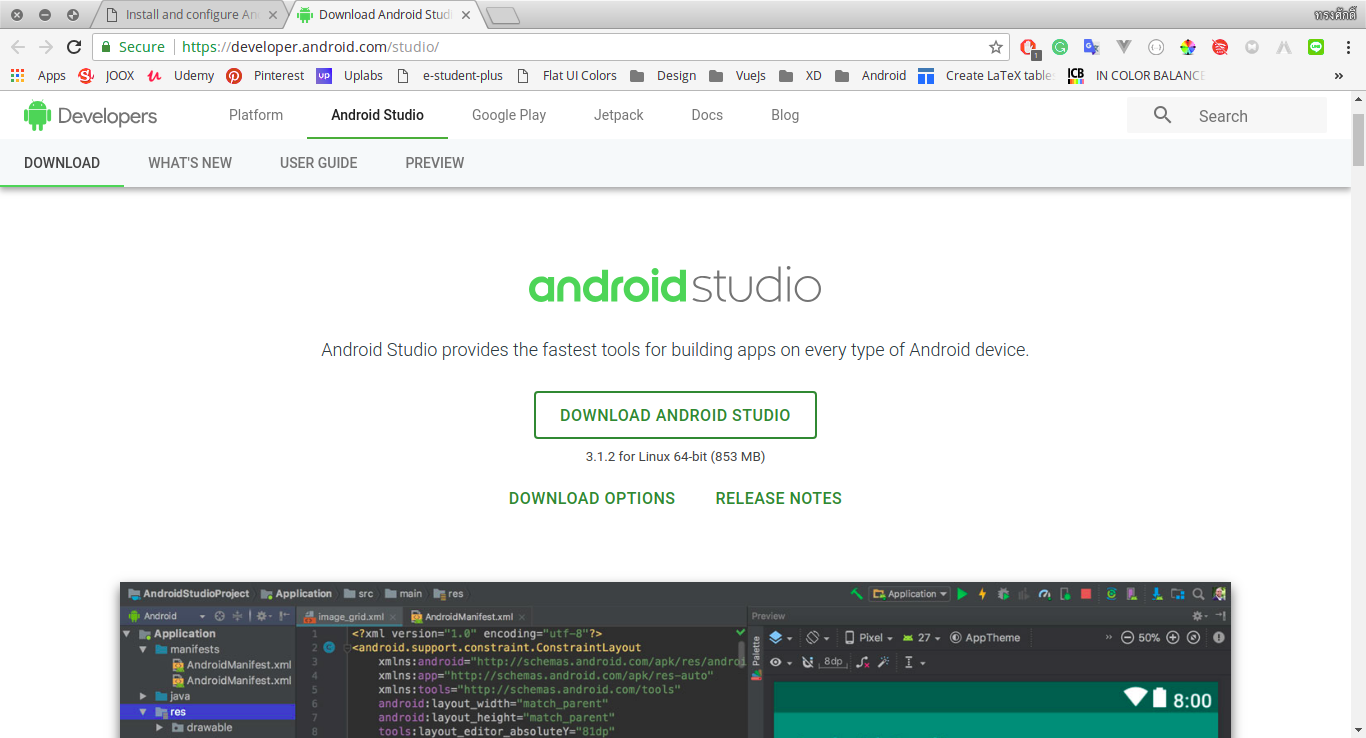
\includegraphics[width=\columnwidth]{Figures/prepareation/android1}
		\caption{หน้าเว็บดาวน์โหลด Android Studio}
		\label{Fig:android1}
	\end{figure}
	
	\item  แสดงหน้าต่างต้อนรับของ  Android Studio ทำการกด Next เพื่อเริ่มกระบวนการติดตั้ง ดังแสดงในรูปที่ \ref{Fig:android2}
	\begin{figure}[H]
		\centering
		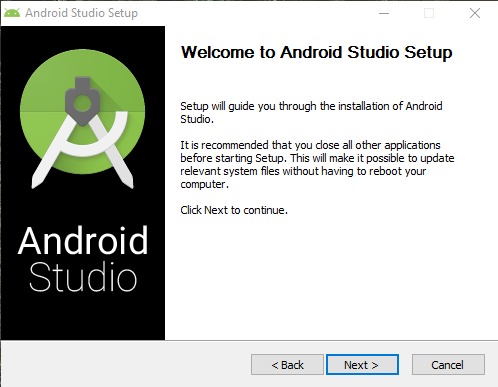
\includegraphics[width=0.7\columnwidth]{Figures/prepareation/android2}
		\caption{หน้าต่างต้อนรับของ  Android Studio}
		\label{Fig:android2}
	\end{figure}
	
	\item  แสดงหน้าต่างข้อตกลงการใช้งาน Android Studio ทำการกด  I Agree ดังแสดงในรูปที่ \ref{Fig:android4}
	\begin{figure}[H]
		\centering
		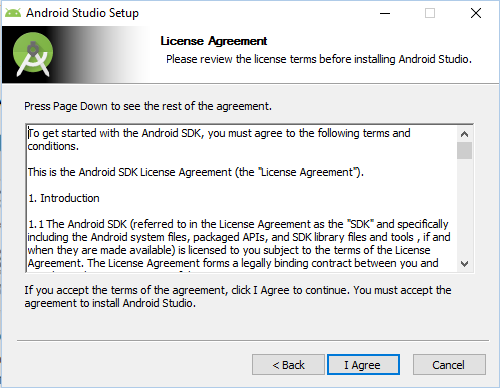
\includegraphics[width=0.7\columnwidth]{Figures/prepareation/android4}
		\caption{หน้าต่างข้อตกลงการใช้งาน  Android Studio}
		\label{Fig:android4}
	\end{figure}
	
	\item  แสดงหน้าต่างที่จัดเก็บไฟล์ต่างๆ ของ Android Studio ทำการกด Next ดังแสดงในรูปที่ \ref{Fig:android5}
	\begin{figure}[H]
		\centering
		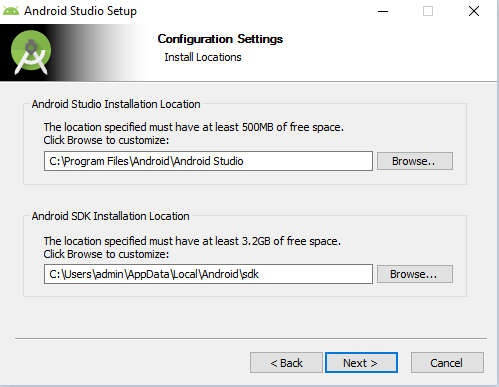
\includegraphics[width=0.7\columnwidth]{Figures/prepareation/android5}
		\caption{หน้าต่างที่จัดเก็บไฟล์ต่างๆ ของ  Android Studio}
		\label{Fig:android5}
	\end{figure}
	
	\item  หน้าต่างเริ่มทำการติดตั้งทำการกด Install ดังแสดงในรูปที่ \ref{Fig:android6}
	\begin{figure}[H]
		\centering
		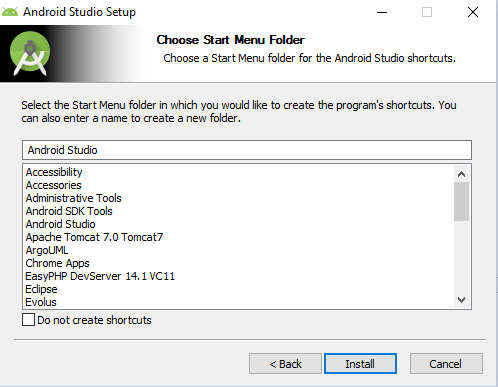
\includegraphics[width=0.7\columnwidth]{Figures/prepareation/android6}
		\caption{หน้าต่างที่จัดเก็บไฟล์ต่างๆ ของ  Android Studio}
		\label{Fig:android6}
	\end{figure}
	
	\item  หน้าต่างผลการติดตั้ง Android Studio ดังแสดงในรูปที่ \ref{Fig:android7}
	\begin{figure}[H]
		\centering
		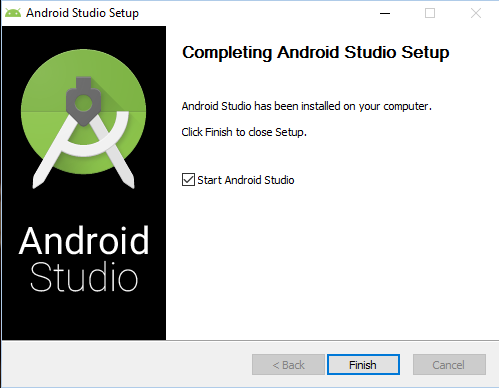
\includegraphics[width=0.7\columnwidth]{Figures/prepareation/android7}
		\caption{ หน้าต่างผลการติดตั้ง Android Studio}
		\label{Fig:android7}
	\end{figure}
	
\end{enumerate}

\section{การติดตั้ง Node.js}
\begin{enumerate}
	\item สามารถดาวน์โหลด Node.js installer package ได้ที่ https://nodejs.org/en/download/ ดังแสดงในรูปที่ \ref{Fig:nodeInstall1}
	\begin{figure}[H]
		
\includegraphics[width=\columnwidth]{Figures/7/1}
		\caption{หน้าเว็บดาวน์โหลด Node.js}
		\label{Fig:nodeInstall1}
	\end{figure}
	
	\item เปิดไฟล์ติดตั้ง ชื่อ node-vx.xx.x-x64.msi เพื่อทำการติดตั้ง ดังแสดงในรูปที่ \ref{Fig:nodeInstall2}
	\begin{figure}[H]
		
\includegraphics[width=\columnwidth]{Figures/7/2}
		\caption{ไฟล์ติดตั้งสำหรับติดตั้ง Node.js}
		\label{Fig:nodeInstall2}
	\end{figure}
	
	\item แสดงหน้าต่างต้อนรับของ Node.js ทำการกด Next เพื่อเริ่มกระบวนการติดตั้ง ดังแสดงในรูปที่ \ref{Fig:nodeInstall3}
	\begin{figure}[H]
		\centering
		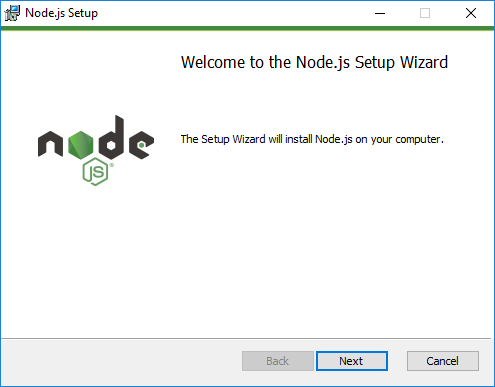
\includegraphics[width=0.7\columnwidth]{Figures/7/3}
		\caption{หน้าต่างตอนรับของ Node.js}
		\label{Fig:nodeInstall3}
	\end{figure}
	
	\item แสดงหน้าต่างข้อตกลงในการใช้ Node.js ให้เลือกช่อง I accept the terms in the License Agreement และกด Next ดังแสดงในรูปที่ \ref{Fig:nodeInstall4}
	\begin{figure}[H]
		\centering
		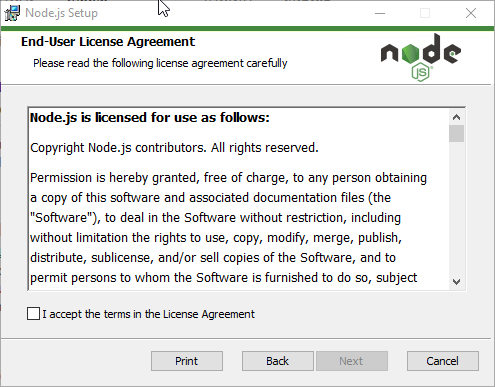
\includegraphics[width=0.7\columnwidth]{Figures/7/4}
		\caption{หน้าต่างข้อตกลงในการใช้ Node.js}
		\label{Fig:nodeInstall4}
	\end{figure}
	
	\item แสดงหน้าต่างเลือกโฟลเดอร์ที่จะทำการติดตั้ง ดังแสดงในรูปที่ \ref{Fig:nodeInstall5}
	\begin{figure}[H]
		\centering
		
\includegraphics[width=0.7\columnwidth]{Figures/7/5}
		\caption{หน้าต่างเลือกโฟลเดอร์ที่จะทำการติดตั้ง Node.js}
		\label{Fig:nodeInstall5}
	\end{figure}
	
	\item แสดงหน้าต่างสำหรับติดตั้ง Node.js ทำการกด Install เพื่อทำการติดตั้ง ดังแสดงในรูปที่ \ref{Fig:nodeInstall6}
	\begin{figure}[H]
		\centering
		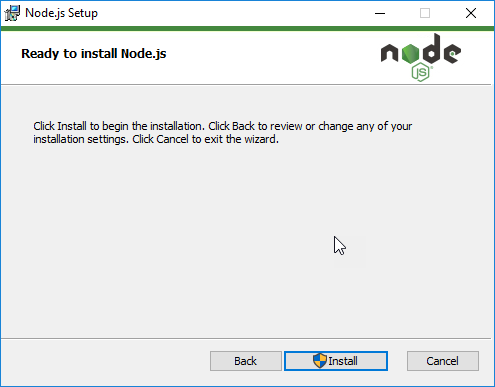
\includegraphics[width=0.7\columnwidth]{Figures/7/6}
		\caption{หน้าต่างติดตั้ง Node.js}
		\label{Fig:nodeInstall6}
	\end{figure}
\end{enumerate}

\section{การติดตั้ง Vue.js Fronted Framwork}
การติดตั้ง Vue.js Fronted Framwork สามารถทำผ่านคำสั่ง command line ได้ โดยจำเป็นต้องทำการติดตั้ง Node.js ก่อนเพื่อใช้ในกระบวนการติดตั้งนี้ ดังแสดงในรูปที่ \ref{Fig:Vue}
\begin{figure}[H]
	{\setstretch{1.0}\begin{lstlisting}[numbers=none]
		npm install -g @vue/cli            
		\end{lstlisting}}
	\caption{คำสั่งสำหรับติดตั้ง Vue.js Fronted Framwork}
	\label{Fig:Vue}
\end{figure}
\newpage
ผลการติดตั้ง Vue.js Fronted Framwork ดังแสดงในรูปที่ \ref{Fig:หน้าต่างผลการติดตั้ง}
\begin{figure}[H]
	\centering
	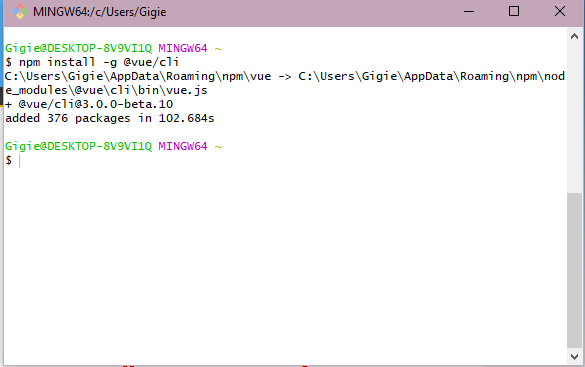
\includegraphics[width=\columnwidth]{Figures/prepareation/vue}
	\caption{หน้าต่างผลการติดตั้ง}
	\label{Fig:หน้าต่างผลการติดตั้ง}
\end{figure}